%%%%%%%%%%%%%%%%%%%%%%%%%%%%%%%%%%%%%%%%%
% Masters/Doctoral Thesis 
% LaTeX Template
% Version 2.5 (27/8/17)
%
% This template was downloaded from:
% http://www.LaTeXTemplates.com
%
% Version 2.x major modifications by:
% Vel (vel@latextemplates.com)
%
% This template is based on a template by:
% Steve Gunn (http://users.ecs.soton.ac.uk/srg/softwaretools/document/templates/)
% Sunil Patel (http://www.sunilpatel.co.uk/thesis-template/)
%
% Template license: 
% CC BY-NC-SA 3.0 (http://creativecommons.org/licenses/by-nc-sa/3.0/)
%
%%%%%%%%%%%%%%%%%%%%%%%%%%%%%%%%%%%%%%%%%

%----------------------------------------------------------------------------------------
%	PACKAGES AND OTHER DOCUMENT CONFIGURATIONS
%----------------------------------------------------------------------------------------

\documentclass[
11pt, % The default document font size, options: 10pt, 11pt, 12pt
%oneside, % Two side (alternating margins) for binding by default, uncomment to switch to one side
english, % ngerman for German
singlespacing, % Single line spacing, alternatives: onehalfspacing or doublespacing
%draft, % Uncomment to enable draft mode (no pictures, no links, overfull hboxes indicated)
%nolistspacing, % If the document is onehalfspacing or doublespacing, uncomment this to set spacing in lists to single
%liststotoc, % Uncomment to add the list of figures/tables/etc to the table of contents
%toctotoc, % Uncomment to add the main table of contents to the table of contents
%parskip, % Uncomment to add space between paragraphs
%nohyperref, % Uncomment to not load the hyperref package
headsepline, % Uncomment to get a line under the header
%chapterinoneline, % Uncomment to place the chapter title next to the number on one line
%consistentlayout, % Uncomment to change the layout of the declaration, abstract and acknowledgements pages to match the default layout
]{MastersDoctoralThesis} % The class file specifying the document structure

\usepackage[utf8]{inputenc} % Required for inputting international characters
\usepackage[T1]{fontenc} % Output font encoding for international characters

\usepackage{mathpazo} % Use the Palatino font by default
\usepackage{tcolorbox} % quote box

\usepackage{float} % place here (H)
\usepackage{subcaption} % subfigures

\usepackage{graphicx} % for table resize
\usepackage{booktabs} % for nice looking tables
\usepackage{lscape} % for landscape tables
\usepackage{longtable} % for multipage tables

\usepackage{listings} % code highlighting
\usepackage{xcolor}
\definecolor{codegreen}{rgb}{0,0.6,0}
\definecolor{codegray}{rgb}{0.5,0.5,0.5}
\definecolor{codepurple}{rgb}{0.58,0,0.82}
\definecolor{backcolour}{rgb}{0.95,0.95,0.92}
\lstdefinestyle{mystyle}{
    backgroundcolor=\color{backcolour},   
    commentstyle=\color{codegreen},
    keywordstyle=\color{magenta},
    numberstyle=\tiny\color{codegray},
    stringstyle=\color{codepurple},
    basicstyle=\ttfamily\footnotesize,
    breakatwhitespace=false,         
    breaklines=true,                 
    captionpos=b,                    
    keepspaces=true,                 
    numbers=left,                    
    numbersep=5pt,                  
    showspaces=false,                
    showstringspaces=false,
    showtabs=false,                  
    tabsize=2
}
\lstset{style=mystyle}


\usepackage[backend=bibtex,style=authoryear,natbib=true]{biblatex} % Use the bibtex backend with the authoryear citation style (which resembles APA)

\addbibresource{references.bib} % The filename of the bibliography

\usepackage[autostyle=true]{csquotes} % Required to generate language-dependent quotes in the bibliography

%----------------------------------------------------------------------------------------
%	MARGIN SETTINGS
%----------------------------------------------------------------------------------------

\geometry{
	paper=a4paper, % Change to letterpaper for US letter
	inner=2.5cm, % Inner margin
	outer=3.8cm, % Outer margin
	bindingoffset=.5cm, % Binding offset
	top=1.5cm, % Top margin
	bottom=1.5cm, % Bottom margin
	%showframe, % Uncomment to show how the type block is set on the page
}

%----------------------------------------------------------------------------------------
%	THESIS INFORMATION
%----------------------------------------------------------------------------------------

\thesistitle{Incremental Snapshotting in Transactional Dataflow SFaaS Systems} % Your thesis title, this is used in the title and abstract, print it elsewhere with \ttitle
\supervisor{Dr. Asterios \textsc{Katsifodimos}} % Your supervisor's name, this is used in the title page, print it elsewhere with \supname
\examiner{} % Your examiner's name, this is not currently used anywhere in the template, print it elsewhere with \examname
\degree{Master of Science} % Your degree name, this is used in the title page and abstract, print it elsewhere with \degreename
\author{Nikolaos \textsc{Gavalas}} % Your name, this is used in the title page and abstract, print it elsewhere with \authorname
\addresses{} % Your address, this is not currently used anywhere in the template, print it elsewhere with \addressname

\subject{Computer Science} % Your subject area, this is not currently used anywhere in the template, print it elsewhere with \subjectname
\keywords{TODO} % Keywords for your thesis, this is not currently used anywhere in the template, print it elsewhere with \keywordnames
\university{\href{http://www.tudelft.nl}{Delft University of Technology}} % Your university's name and URL, this is used in the title page and abstract, print it elsewhere with \univname
\department{\href{https://www.tudelft.nl/en/eemcs/the-faculty/departments/software-technology/}{Software Technology}} % Your department's name and URL, this is used in the title page and abstract, print it elsewhere with \deptname
\group{\href{http://www.wis.ewi.tudelft.nl/}{Web Information Systems Group}} % Your research group's name and URL, this is used in the title page, print it elsewhere with \groupname
\faculty{\href{https://www.tudelft.nl/en/ewi/}{Electrical Engineering, Mathematics and Computer Science}} % Your faculty's name and URL, this is used in the title page and abstract, print it elsewhere with \facname

\AtBeginDocument{
\hypersetup{pdftitle=\ttitle} % Set the PDF's title to your title
\hypersetup{pdfauthor=\authorname} % Set the PDF's author to your name
\hypersetup{pdfkeywords=\keywordnames} % Set the PDF's keywords to your keywords
}

\begin{document}

\frontmatter % Use roman page numbering style (i, ii, iii, iv...) for the pre-content pages

\pagestyle{plain} % Default to the plain heading style until the thesis style is called for the body content

%----------------------------------------------------------------------------------------
%	TITLE PAGE
%----------------------------------------------------------------------------------------

\begin{titlepage}
\begin{center}

\vspace*{.06\textheight}
{\scshape\LARGE \univname\par}\vspace{1.5cm} % University name
\textsc{\Large Masters Thesis}\\[0.5cm] % Thesis type

\HRule \\[0.4cm] % Horizontal line
{\huge \bfseries \ttitle\par}\vspace{0.4cm} % Thesis title
\HRule \\[1.5cm] % Horizontal line
 
\begin{minipage}[t]{0.4\textwidth}
\begin{flushleft} \large
\emph{Author:}\\
\href{http://www.johnsmith.com}{\authorname} % Author name - remove the \href bracket to remove the link
\end{flushleft}
\end{minipage}
\begin{minipage}[t]{0.4\textwidth}
\begin{flushright} \large
\emph{Supervisor:} \\
\href{http://www.jamessmith.com}{\supname} % Supervisor name - remove the \href bracket to remove the link  
\end{flushright}
\end{minipage}\\[3cm]
 
\vfill

\large \textit{A thesis submitted in fulfillment of the requirements\\ for the degree of \degreename}\\[0.3cm] % University requirement text
\textit{in the}\\[0.4cm]
\groupname\\\deptname\\[2cm] % Research group name and department name
 
\vfill

{\large \today}\\[4cm] % Date
%\includegraphics{Logo} % University/department logo - uncomment to place it
 
\vfill
\end{center}
\end{titlepage}

%----------------------------------------------------------------------------------------
%	DECLARATION PAGE
%----------------------------------------------------------------------------------------

% \begin{declaration}
% \addchaptertocentry{\authorshipname} % Add the declaration to the table of contents
% \noindent I, \authorname, declare that this thesis titled, \enquote{\ttitle} and the work presented in it are my own. I confirm that:

% \begin{itemize} 
% \item This work was done wholly or mainly while in candidature for a research degree at this University.
% \item Where any part of this thesis has previously been submitted for a degree or any other qualification at this University or any other institution, this has been clearly stated.
% \item Where I have consulted the published work of others, this is always clearly attributed.
% \item Where I have quoted from the work of others, the source is always given. With the exception of such quotations, this thesis is entirely my own work.
% \item I have acknowledged all main sources of help.
% \item Where the thesis is based on work done by myself jointly with others, I have made clear exactly what was done by others and what I have contributed myself.\\
% \end{itemize}
 
% \noindent Signed:\\
% \rule[0.5em]{25em}{0.5pt} % This prints a line for the signature
 
% \noindent Date:\\
% \rule[0.5em]{25em}{0.5pt} % This prints a line to write the date
% \end{declaration}

\cleardoublepage

%----------------------------------------------------------------------------------------
%	QUOTATION PAGE
%----------------------------------------------------------------------------------------

% \vspace*{0.2\textheight}

% \noindent\enquote{\itshape Thanks to my solid academic training, today I can write hundreds of words on virtually any topic without possessing a shred of information, which is how I got a good job in journalism.}\bigbreak

% \hfill Dave Barry

%----------------------------------------------------------------------------------------
%	ABSTRACT PAGE
%----------------------------------------------------------------------------------------

\begin{abstract}
\addchaptertocentry{\abstractname} % Add the abstract to the table of contents
TODO
\end{abstract}

%----------------------------------------------------------------------------------------
%	ACKNOWLEDGEMENTS
%----------------------------------------------------------------------------------------

\begin{acknowledgements}
\addchaptertocentry{\acknowledgementname} % Add the acknowledgements to the table of contents
TODO
\end{acknowledgements}

%----------------------------------------------------------------------------------------
%	LIST OF CONTENTS/FIGURES/TABLES PAGES
%----------------------------------------------------------------------------------------

\tableofcontents % Prints the main table of contents

\listoffigures % Prints the list of figures

\listoftables % Prints the list of tables

%----------------------------------------------------------------------------------------
%	ABBREVIATIONS
%----------------------------------------------------------------------------------------

% \begin{abbreviations}{ll} % Include a list of abbreviations (a table of two columns)

% \textbf{LAH} & \textbf{L}ist \textbf{A}bbreviations \textbf{H}ere\\
% \textbf{WSF} & \textbf{W}hat (it) \textbf{S}tands \textbf{F}or\\

% \end{abbreviations}

%----------------------------------------------------------------------------------------
%	PHYSICAL CONSTANTS/OTHER DEFINITIONS
%----------------------------------------------------------------------------------------

% \begin{constants}{lr@{${}={}$}l} % The list of physical constants is a three column table

% % The \SI{}{} command is provided by the siunitx package, see its documentation for instructions on how to use it

% Speed of Light & $c_{0}$ & \SI{2.99792458e8}{\meter\per\second} (exact)\\
% %Constant Name & $Symbol$ & $Constant Value$ with units\\

% \end{constants}

%----------------------------------------------------------------------------------------
%	SYMBOLS
%----------------------------------------------------------------------------------------

% \begin{symbols}{lll} % Include a list of Symbols (a three column table)

% $a$ & distance & \si{\meter} \\
% $P$ & power & \si{\watt} (\si{\joule\per\second}) \\
% %Symbol & Name & Unit \\

% \addlinespace % Gap to separate the Roman symbols from the Greek

% $\omega$ & angular frequency & \si{\radian} \\

% \end{symbols}

%----------------------------------------------------------------------------------------
%	DEDICATION
%----------------------------------------------------------------------------------------

% \dedicatory{For/Dedicated to/To my\ldots}

%----------------------------------------------------------------------------------------
%	THESIS CONTENT - CHAPTERS
%----------------------------------------------------------------------------------------

\mainmatter % Begin numeric (1,2,3...) page numbering

\pagestyle{thesis} % Return the page headers back to the "thesis" style

% Include the chapters of the thesis as separate files from the Chapters folder
% Uncomment the lines as you write the chapters

%!TEX root = ../main.tex

\chapter{Introduction}

\label{Chapter1}

Cloud Computing has seen a dramatic rise in its adoption the recent years, with an increasing number of enterprises migrating their software and hardware to the cloud, and this trend is only expected to continue [\cite{serverless-preds}].
Historically, this shift towards managed infrastructure has been arguably inevitable, because with cloud computing the cost per unit of computation is minimized [\cite{rise-of-serverless}].
The drive for increased efficiency in computation has culminated in the emergence of the \textit{serverless} architecture [\cite{serverless-definition}].

In the serverless cloud computing execution model, applications are being developed as collections of fine-grained event-driven and stateless units of computation called \textit{cloud functions}.
Cloud providers offer the execution of serverless functions as a paid service, known as \textit{Function-as-a-Service} or \textit{FaaS} [\cite{faas-definition}].

While FaaS offerings prioritize scalability by being stateless, most applications require some form of state management, resulting in developers resorting to external databases for their applications' state-keeping.
Several recent works have aimed to alleviate the burden of state management from application developers [\cite{orleans,durable-functions,beldi}] by enabling the transparent management of application state through external databases, thereby providing \textit{stateful functions}, or \textit{SFaaS}.

SFaaS systems ease the development of stateful applications, but they are not a panacea per se.
Any programmer that develops distributed applications will eventually have to deal with fundamental potential issues such as network partitioning, system failures and the Byzantine generals messaging problem [\cite{byzantine}].
These problems become especially hard to deal with when the application level requires implementing \textit{transactional} logic, as transactions require extra guarantees. Transactions are sets of operations that must adhere to the ACID principles - Atomicity, Consistency, Isolation, and Durability [\cite{transaction-definition}]. 

Consequently, developers often find themselves intermixing business logic with consistency checks, rollbacks, snapshots, and timeouts, resulting in systems that are highly intricate to maintain and prone to failures. This highlights the need for an intermediary layer that abstracts the distributed fault-tolerance logic and provides application developers with specific guarantees, both at the state-management level and the transactional level, if feasible.

SFaaS systems built on top of \textit{stateful streaming dataflow engines} such as Apache Flink StateFun [\cite{apache-flink}] make excellent candidates for implementing \textit{transactional SFaaS} systems, primarily for two reasons [\cite{transactions-serverless-functions-leveraging-stateful-dataflows}]:

\begin{enumerate}
    \item They offer \textit{exactly-once} message delivery semantics, eliminating the need for identifying lost messages and resending them, and also guarantee the message delivery order - the communication channels between the distributed components are FIFO.

    \item They fully manage the system's global distributed state by periodically creating consistent snapshots and recovering them upon failures. This is especially important for implementing transactions, since for failed transactions there needs to be a rollback mechanism to guarantee the Atomicity property.
\end{enumerate}

Dataflow SFaaS systems are comprised of multiple worker processes, with each of them keeping a partition of the global state locally [\cite{apache-flink}]. The state is represented as key-value pairs, making key-value stores an ideal choice as embedded databases for this task.

As the key-value store is a critical component of this architecture, it is essential to carefully evaluate the available options of suitable types of key-value stores and motivate our selection. Towards this end, in this study, we implement three different kinds of key-value stores, evaluate their performance within transactional dataflow systems and conduct a comprehensive comparative analysis among them.

\section{Design Requirements}
\label{design-requirements}

In a (transactional) dataflow SFaaS system, the key-value stores need to have specific properties to be considered suitable. These properties, extending those mentioned in the work of \cite{faster}, are:

\begin{enumerate}
    \item \textit{Incremental snapshots} [\cite{state-management-apache-flink}].
    When the dataflow engine requests a worker to create a snapshot of its state, the state backend (the key-value store) will dump the state and save it. As this process happens many times during the execution of a workflow, to ensure fault-tolerance and fast state recovery, it is imperative that it is done efficiently, building on previous snapshots.
    
    The naive solution is to save the whole state every time, but if there is a way to only save the updates on the state at each step, incrementally, it would definitely be more efficient. However, saving only the updates on each step, would make recovery very slow, as the state would need to be rebuilt from the very beginning in case of a system failure.
    In this work, we propose a solution that combines \textit{fast incremental snapshots with low recovery times}.

    \item \textit{State recovery to a previous version from previous snapshots (rollback)} [\cite{snapshots-rollbacks,state-management-apache-flink}]. Upon execution, the dataflow coordinator process may request the workers to restore some previous version of their state, so that the system can go back to some consistent global state and ``replay'' events to recover from some failure.
    
    \item \textit{Larger-than-memory data (spill-to-disk)}.
    When dealing with large volumes of data, it is expected that during execution the state will exceed in size the amount that can be stored in memory.
    Hence, it is essential that the key-value store employs persistent storage when necessary to handle states larger than the available memory.

    \item \textit{Update-intensity}.
    In dataflow systems, changes to the state are typically characterized by the volume of updates rather than inserts or deletes.
    This is particularly evident in workflows that involve data aggregations or analytics, and it holds even more significance in systems that support transactions.
    Transactional systems often involve frequent operations like value increments. As a result, the state backend needs to be well-suited for update-heavy workloads.

    \item \textit{Locality}.
    In real-world dataflow applications, access to data is rarely uniformly distributed.
    Keys that are ``alive'' at any moment may be of many orders of magnitude, but it's usually a subset of those that are ``hot'' at some given time, i.e. accessed or updated frequently.
    The hot set may drift as time passes but the strong temporal locality property is maintained.

    \item \textit{Point operations}.
    A key-value store for our use-case should be optimal for point operations, i.e. operations associated with a single key, as opposed to range operations.
    Since state updates rarely operate on ranges of keys, we can leverage this knowledge to our advantage.

    % TODO analytics readiness? - TODO sta future extensions: analytics readiness mporei na epiteuxthei an eixa tombstones giati tote tha mporousa na skanarw osa arxeia thelw xwris na xreiazetai index (=mnhmh). To tombstone tha mpaine se record metadata, sta opoia tha mporousa na valw kai kapoio checksum, kapoio crc gia na mai sigouros oti to record den einai corrupted.
\end{enumerate}

\section{Research Questions}
\label{section-reseach-questions}

At this juncture we can outline the main research questions of this work. The first research question is:\\

\begin{tcolorbox}
    Which type or types of key-value stores are more fitting as embedded state stores in the worker processes of transactional dataflow SFaaS systems?
\end{tcolorbox}

\vspace{8px}
To address this question in alignment with the design requirements outlined in subsection \ref{design-requirements}, our approach involves several steps.
Firstly, we will survey and examine existing key-value store designs, considering their suitability for our purposes.
Next, we will carefully narrow down our options and provide a compelling rationale for our chosen selections.
Subsequently, we will proceed to implement the most promising candidates, and study them in depth, which leads us to the second and third research questions:\\

\begin{tcolorbox}
    How do changes in the parameters of each selected type of key-value store affect its performance?
\end{tcolorbox}
\vspace{8px}

\begin{tcolorbox}
    In the selected types of key-value stores, which are the trade-offs that determine their operation? In which general use-cases does each of them perform better?
\end{tcolorbox}
\vspace{8px}

Next, we will proceed with a thorough evaluation of the implemented key-value stores by integrating them into a transactional dataflow system. During this evaluation, we will specifically focus on assessing the efficiency of the incremental snapshotting functionality and its impact. Thus, our fourth research question is formulated as follows:\\

\begin{tcolorbox}
    How does the performance of a key-value store that incorporates incremental snapshotting functionality compare to that of a "naive" in-memory key-value store, which captures snapshots of its entire state at each step, in terms of snapshot creation time?
\end{tcolorbox}
\vspace{8px}

Ultimately, we will be able to address the final research question:\\

\begin{tcolorbox}
    Is there a key-value store that clearly stands out as the superior choice for state management?
    % TODO spoiler alert no, offer the programmer the ability to choose based on his app's reqs
\end{tcolorbox}
\vspace{8px}

\section{Contributions}

We summarize this work's contributions in the following points:

\begin{enumerate}
    \item \textit{Design and implementation of Three Key-Value Stores}: To ensure a fair comparison and level playing field, we have implemented three distinct key-value store implementations. Each implementation adheres to the same programming language and incorporates similar design choices for shared functionality, such as data encoding and data structures. By keeping these aspects consistent, we can isolate the differences in the key-value store logic and facilitate accurate comparisons.
    
    \item \textit{Experimental Analysis}: In order to address the research questions outlined in section \ref{section-reseach-questions}, we have conducted a series of experiments. These experiments focus on analyzing the parameters of each implemented key-value store and exploring the trade-offs inherent in their designs, particularly in terms of resource utilization. By systematically examining these aspects, we aim to gain a deeper understanding of the strengths and weaknesses of each key-value store implementation.

    \item \textit{Comprehensive Comparison}: Building upon the experimental analysis, we have conducted a comprehensive comparison among the implemented key-value. This comparison encompasses various factors, including the effectiveness of incremental snapshotting, which plays a vital role in state management. Ultimately, our goal is to determine whether one key-value store emerges as the optimal choice for our specific use case. By thoroughly evaluating the performance and capabilities of each implementation, we aim to provide insights and make informed recommendations for state management in transactional dataflow systems.
\end{enumerate}

\section{Outline}

The rest of the thesis is structured as follows:

Chapter \ref{Chapter2-related-work} provides a review of the existing literature and related work in the field. It explores previous research, methodologies, and advancements in key-value stores and state management within transactional dataflow systems. This chapter establishes a solid foundation for our own study.

In chapter \ref{Chapter3-implementation}: we delve into comprehensive descriptions of the internal workings of each type of key-value store. We provide in-depth insights into their underlying mechanisms, data structures, and algorithms. Furthermore, we discuss the specific implementation details and design decisions that pertain to each key-value store type. By thoroughly understanding the intricacies of each implementation, we lay the groundwork for subsequent evaluations and comparisons.

Chapter \ref{Chapter4-evaluation} is dedicated to the evaluation of our implemented key-value stores. We conduct a series of benchmarks and comparisons to assess their performance and capabilities. This includes integrating the key-value stores into a transactional dataflow system to simulate real-world usage scenarios. By rigorously evaluating their performance, scalability, and efficiency, we gain valuable insights into the strengths and limitations of each implementation. We discuss the obtained results and analyze the implications they have on state management in transactional dataflow systems.

In the final chapter, \ref{Chapter5-conclusion}, we provide a comprehensive summary of our research and findings. We present our conclusions based on the evaluation and comparisons performed. We also address the research questions posed earlier in the thesis and provide insightful answers. Additionally, we discuss potential directions for future research and highlight areas that require further exploration and development.
% TODO and mention the limitations of this work?

%!TEX root = ../main.tex

\chapter{Related Work} % Main chapter title

\label{Chapter2-related-work}

\section{TODO}

% related work: https://www.sciencedirect.com/science/article/pii/S0306437922000229?ref=pdf_download&fr=RR-2&rr=7c0f0989de86b7af

% faster

% LSM tree -> cassandra/rocksdb

% find some paper for bitcask kvstore

% fractal trees

% In support of workload-aware streaming state management

% JSON crdt?

% Lightweight Asynchronous Snapshots for Distributed Dataflows

%% **** state management in apache flink section 4.2!!

% for transactional sfaas check the transactions across serverless functions leveraging.. .paper


% There are several types of disk-based key-value stores available, including:

% LevelDB: A popular open-source key-value store that is optimized for read-heavy workloads and has a small memory footprint.

% RocksDB: A fork of LevelDB that is designed to handle a wider range of workloads, including write-heavy ones.

% LMDB: A high-performance, memory-mapped key-value store that supports multi-threading and transactions.

% Cassandra: A distributed key-value store that is optimized for write-heavy workloads and provides tunable consistency levels.

% Riak: A distributed key-value store that is designed for high availability and fault-tolerance and supports both eventual and strong consistency.

% Berkeley DB: A mature and battle-tested embedded key-value store that supports transactions, replication, and high availability.

% Kyoto Cabinet: An efficient and lightweight key-value store that is designed for high-speed data storage and retrieval.

% Redis: A popular in-memory key-value store that also provides disk-based persistence, making it suitable for large datasets that cannot fit in memory.




% NOTE - including 2 images side by side before i forget

% \begin{figure}[H]
%     \begin{subfigure}{.5\textwidth}
%         \centering
%         \includegraphics[width=0.8\linewidth]{1a.png}
%         \caption{NN}
%         \label{fig:1a}
%     \end{subfigure}
%     \begin{subfigure}{.5\textwidth}
%         \centering
%         \includegraphics[width=0.8\linewidth]{1b.png}
%         \caption{Tri-linear}
%         \label{fig:1b}
%     \end{subfigure}
%     \caption{Tri-linear vs Nearest Neighbours Interpolation}
%     \label{fig:1}
% \end{figure}

% inserting images in general: https://www.overleaf.com/learn/latex/Inserting_Images
 
%!TEX root = ../main.tex

\chapter{Implementation}

\label{Chapter3}

\section{Log-Structured Merge-Tree}

% LSMT with size-tiered compaction (write-optimized)

% explain how it works

% possible optimizations:
% 1. https://www.youtube.com/watch?v=b6SI8VbcT4w
% 2. fence pointers can be used to organize data into compressible blocks
% 3. the .filter and .pointers files could be embedded to the runfile (and then do a relative seek from the end)
% this would help with the save to replica things


\section{Append Log}



\section{Hybrid Log}

% possible extensions/optimizations applicable to all engines:
% concurrency! explain how it can be applied, what to lock etc.
% mmap for the files
% checksums for malformed records

%!TEX root = ../main.tex

\chapter{Evaluation}

\label{Chapter4-evaluation}

% TODO write some intro here

\section{Parameters}

Each of our implemented key-value stores is instantiated with a set of parameters. In Chapter \ref{Chapter3-implementation} we explained what each parameter represents, but to be able to understand the trade-offs among them, and how various settings of them influence the behaviour of the respective engine, it is important to explore them visually.

In this section, the experiments performed aim to highlight qualitatively the effect of each parameter and do not constitute stress tests.

For the following demonstrations, we use by default - unless explicitly stated otherwise - the following settings: The randombly generated keys and values have length 4 bytes, the sets of available keys and values have cardinality $10^3$ each, the distribution of picking keys and values from the sets is uniform, the input write and read throughput are $10^3$ writes and $10^3$ reads per second respectively, and for latency measurements that are sampled (to calculate the 50th and the 95th percentile), the number of samples is 10. Also, for the LSM-Tree we use \verb"max_runs_per_level="3, \verb"memtable_bytes_limit="$10^3$, \verb"density_factor="10, and for the parameters of HybridLog we use \verb"mem_segment_len="$10^4$, \verb"ro_lag_interval="$10^3$, \verb"flush_interval="$10^3$, and \verb"compaction_enabled=False".

\subsection{LSM-Tree}

\subsubsection{Max Runs per Level}

The first parameter of the LSM-Tree is \verb"max_runs_per_level". This controls the maximum amount of runs allowed in a level. As explained in Chapter \ref{Chapter3-implementation}, as the number of runs per level increases, a log-structured database becomes write-optimized, and when it is kept close to 1, the database is optimized for reads. In figure \ref{fig:max-runs-per-level} we demonstrate this behaviour:

\begin{figure}[h]
    \begin{subfigure}{.5\textwidth}
        \centering
        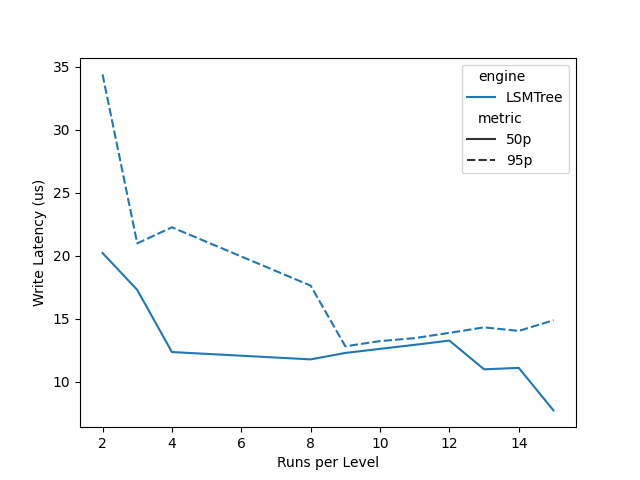
\includegraphics[width=1.1\linewidth]{max_runs_per_level_write.png}
    \end{subfigure}
    \begin{subfigure}{.5\textwidth}
        \centering
        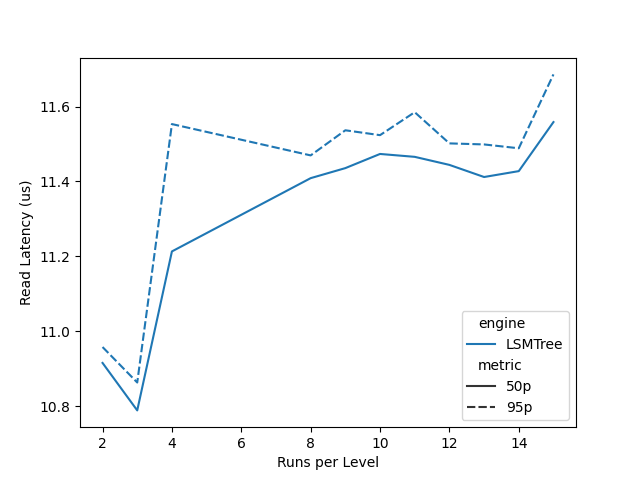
\includegraphics[width=1.1\linewidth]{max_runs_per_level_read.png}
    \end{subfigure}
    \caption{Latency vs Max Runs per Level.}
    \label{fig:max-runs-per-level}
\end{figure}

Clearly, the write latency drops, when \verb"max_runs_per_level" increases, and the read latency is low when the parameter is relatively small.

The LSM-Tree behaves as expected due to the following reasons: when the number of runs per level increases, the log-structuring scheme degrades into a large fragmented log spread over several smaller logs with infrequent merges. This essentially becomes a large log, enabling the maximum writing speed. However, at the same time, accessing a key requires searching through multiple runs per level, leading to slower reads.

This parameter is central, and relevant not only to the LSM-Tree but to the other two log-structured engines, HybridLog and AppendLog. More specifically, the effect on the write latency on these two is the same, but not quite so for the read latency. Because of the fundamental difference in indexing (the latter two use in-memory hash-based indices that point directly to files and offsets), the read latencies are not affected. One needs to just keep the parameter ``balanced'' enough so that then merges are not very large and infrequent, which would impact the overall performance of the stores.

\subsubsection{Density Factor}
The \verb"density_factor", as explained in section \ref{subsection-lsm-design}, controls the width of gaps between the fence pointers of the LSM-Tree.

\begin{figure}[h]
    \begin{subfigure}{.5\textwidth}
        \centering
        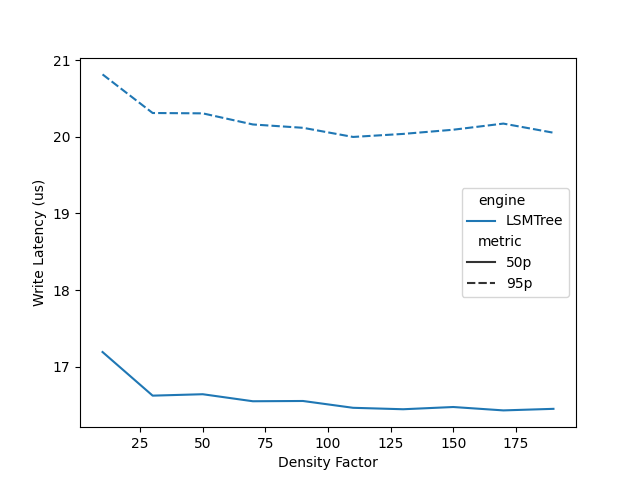
\includegraphics[width=1.1\linewidth]{density_factor_write.png}
    \end{subfigure}
    \begin{subfigure}{.5\textwidth}
        \centering
        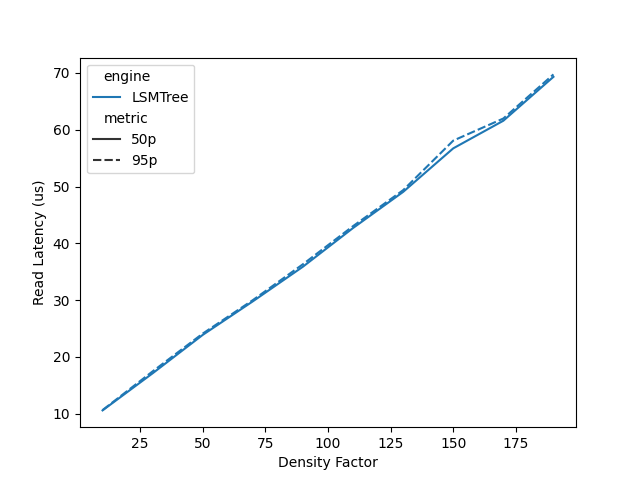
\includegraphics[width=1.1\linewidth]{density_factor_read.png}
    \end{subfigure}
    \caption{Latency vs Density Factor.}
    \label{fig:density_factor_write_read}
\end{figure}

\begin{figure}[h]
    \begin{subfigure}{.5\textwidth}
        \centering
        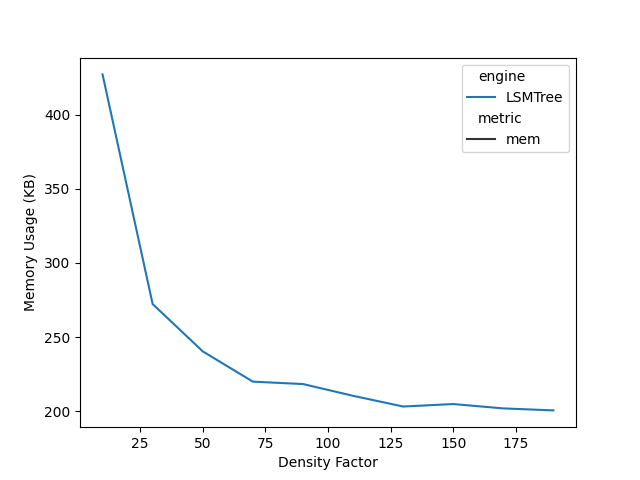
\includegraphics[width=1.1\linewidth]{density_factor_mem.png}
    \end{subfigure}
    \begin{subfigure}{.5\textwidth}
        \centering
        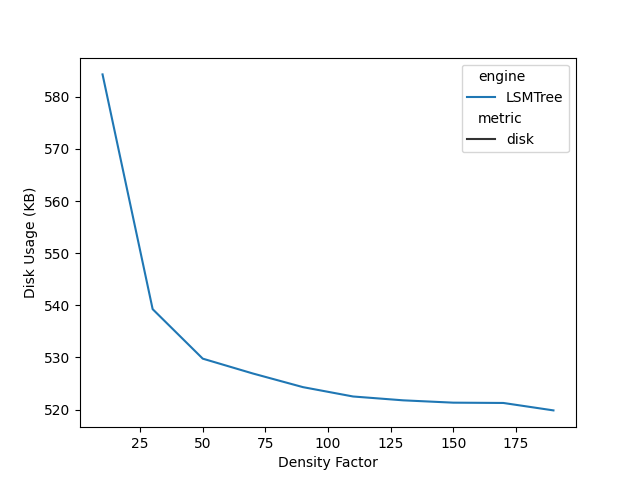
\includegraphics[width=1.1\linewidth]{density_factor_disk.png}
    \end{subfigure}
    \caption{Memory and Disk Usage vs Density Factor.}
    \label{fig:density_factor_mem_disk}
\end{figure}

In figure \ref{fig:density_factor_write_read} we observe the following: as the density factor increases, the writes remain virtually unaffected, and reads become drastically slower. This is because the LSM-Tree, when the density factor is high and therefore the gaps within the offsets are large, has to go through more bytes in the file to find the requested key, which slows down the reads.

However, there is an obvious tension here: we cannot keep the density factor too small, because that would result in higher memory and disk usage, as demonstrated in figure \ref{fig:density_factor_mem_disk}.

\subsubsection{Memtable Size}

The size of the LSM-Tree's memtable, controlled by the \verb"memtable_bytes_limit", is the amount of bytes the in-memory structure can hold before it flushes to disk.

\begin{figure}[h]
    \begin{subfigure}{.5\textwidth}
        \centering
        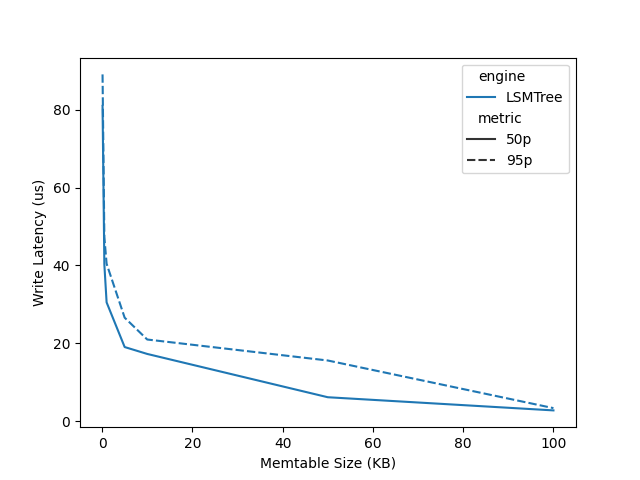
\includegraphics[width=1.1\linewidth]{memtable_bytes_limit_write.png}
    \end{subfigure}
    \begin{subfigure}{.5\textwidth}
        \centering
        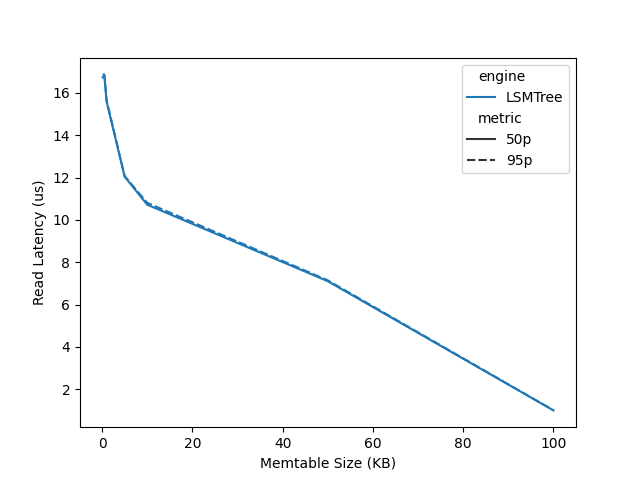
\includegraphics[width=1.1\linewidth]{memtable_bytes_limit_read.png}
    \end{subfigure}
    \caption{Latency vs Memtable Size.}
    \label{fig:memtable-bytes-limit-write-read}
\end{figure}

\begin{figure}[h]
    \centering
    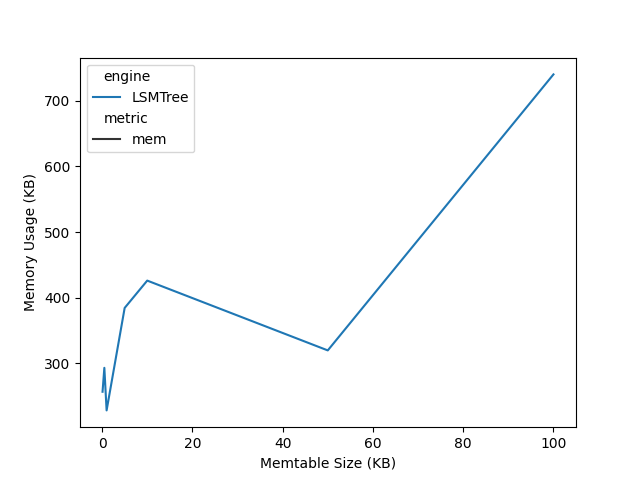
\includegraphics[width=0.6\textwidth]{memtable_bytes_limit_mem.png}
    \caption{Memory Usage vs Memtable Size}
    \label{fig:memtable_bytes_limit_mem}
\end{figure}

In figure \ref{fig:memtable-bytes-limit-write-read} we notice that as the size of the memtable increases, the latency of both the writes and reads drops. This is expected, as with bigger memtables, the probability of accessing a key without the need to reach to the disk is higher. However, the memory usage obviously goes up, as seen in figure \ref{fig:memtable_bytes_limit_mem}, and thus we cannot keep this parameter too large.

\subsection{HybridLog}

\subsubsection{Memory Segment Size}

Besides the indices, HybridLog also keeps a memory segment in memory, which is essentially a ring buffer. The parameter \verb"mem_segment_len" controls the size of this segment. In figure \ref{fig:mem_segment_len_write_read} we see its influence in the latencies of the writes and the reads, and in figure \ref{fig:mem_segment_len_mem.png} we see the memory usage.

\begin{figure}[h]
    \begin{subfigure}{.5\textwidth}
        \centering
        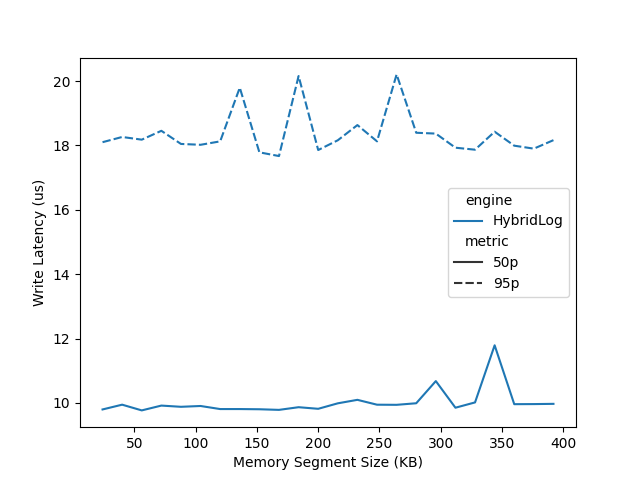
\includegraphics[width=1.1\linewidth]{mem_segment_len_write.png}
    \end{subfigure}
    \begin{subfigure}{.5\textwidth}
        \centering
        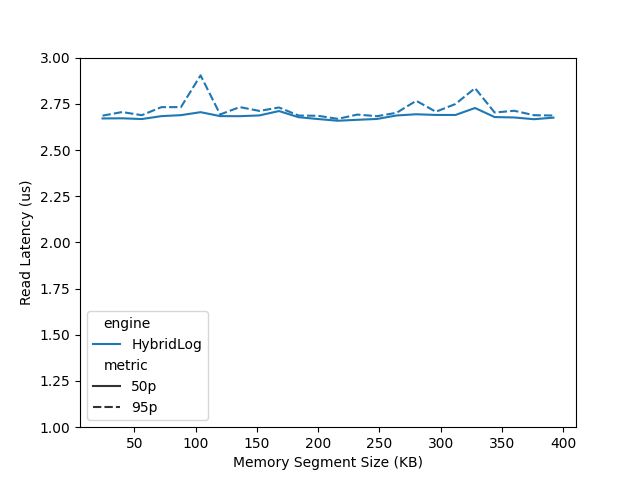
\includegraphics[width=1.1\linewidth]{mem_segment_len_read.png}
    \end{subfigure}
    \caption{Latency vs Memory Segment Length.}
    \label{fig:mem_segment_len_write_read}
\end{figure}


\begin{figure}[h]
    \centering
    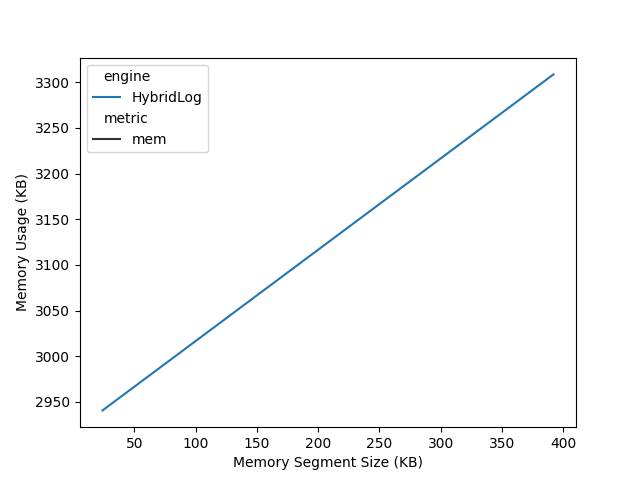
\includegraphics[width=0.6\textwidth]{mem_segment_len_mem.png}
    \caption{Memory Usage vs Memory Segment Size}
    \label{fig:mem_segment_len_mem.png}
\end{figure}

As expected, the size of the in-memory segment is irrelevant to the speed of both writes and reads, while it directly affects the memory used by the engine. It is irrelevant to the latencies because, as we will see later, it is the \verb"ro_lag_interval" which actually matters.

Hence, it is important that we keep this parameter as low as possible. Since it must always hold that the size of the memory segment is larger than the sum of the sizes of the sub-segments defined by \verb"ro_lag_interval" and \verb"flush_interval", this parameter should ideally be set a value slightly larger than the sum of these two intervals.

\subsubsection{Read-only Segment Size}

The read-only segment size is controlled via the value of \verb"ro_lag_interval". Contrary to the memory segment size, this is the parameter which actually influences directly the probability of an in-memory hit of a key lookup, and thus the cache-like behaviour of the whole memory segment.

If this value is big, we expect many in-memory hits, therefore better performance for both writes and reads. This is exactly what we observe in figure \ref{fig:ro_lag_interval}.

\begin{figure}[h]
    \begin{subfigure}{.5\textwidth}
        \centering
        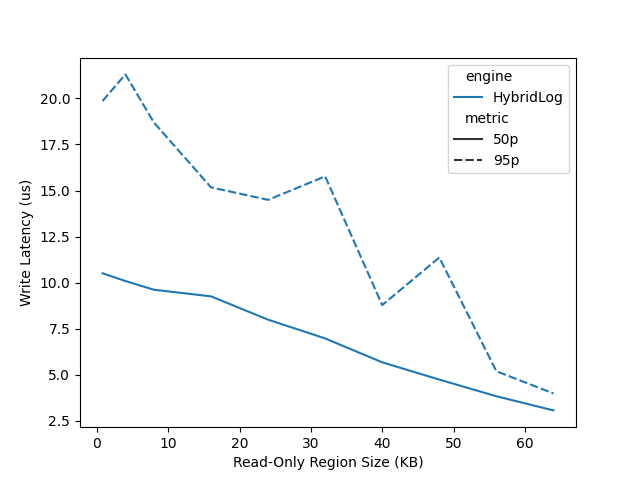
\includegraphics[width=1.1\linewidth]{ro_lag_interval_write.png}
    \end{subfigure}
    \begin{subfigure}{.5\textwidth}
        \centering
        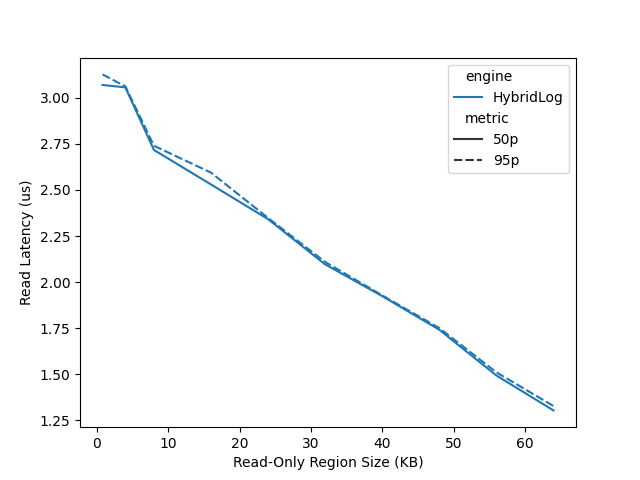
\includegraphics[width=1.1\linewidth]{ro_lag_interval_read.png}
    \end{subfigure}
    \caption{Latency vs Read-only Segment Size.}
    \label{fig:ro_lag_interval}
\end{figure}

\subsubsection{Flush Segment Size}

The flush segment, whose size is adjusted via the \verb"flush_interval" parameter, contains read-only entries that are ready to be flushed to disk. The bigger the segment, the less the probability for disk access and therefore the higher the performance of the key-value store. This is evident in figure \ref{fig:flush_interval_write_read}. The obvious trade-off present here, is that if this value is set to be large, we require a larger memory segment size, which will use more memory.


Additionally, it is crucial to ensure that the value is not set too low. If it is set too low, it may impede the speedup of performance from large flushes to disk, which occur sequentially and are therefore fast. Furthermore, setting the value too low may result in numerous small logs that require frequent merges, thus adversely impacting performance. This phenomenon is also illustrated in the same figure \ref{fig:flush_interval_write_read}.

\begin{figure}[h]
    \begin{subfigure}{.5\textwidth}
        \centering
        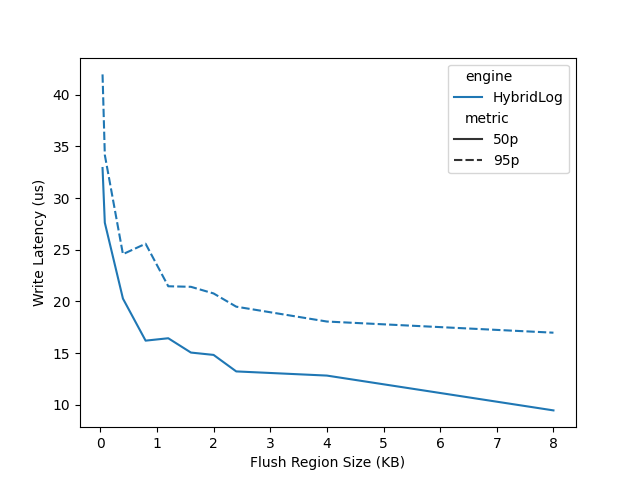
\includegraphics[width=1.1\linewidth]{flush_interval_write.png}
    \end{subfigure}
    \begin{subfigure}{.5\textwidth}
        \centering
        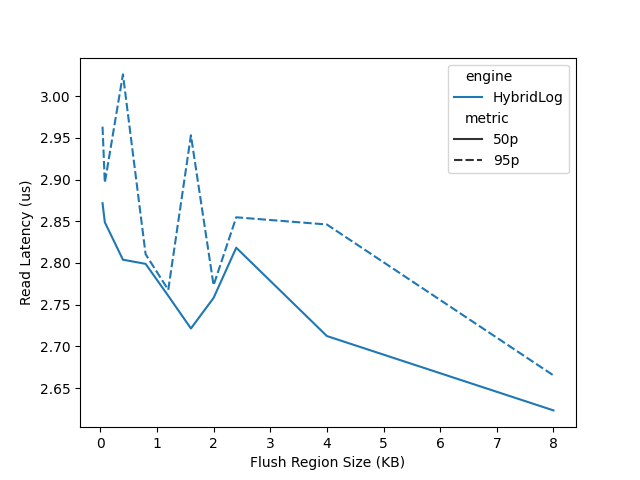
\includegraphics[width=1.1\linewidth]{flush_interval_read.png}
    \end{subfigure}
    \caption{Latency vs Flush Segment Size.}
    \label{fig:flush_interval_write_read}
\end{figure}

\subsubsection{Compaction}

Regarding compaction, one may wonder if it could offer some speedup in practice, since it could be the case that its potential benefit is implicitly provided during merging already, and the system is just wasting time doing extra unnecessary work.

\begin{figure}[h]
    \centering
    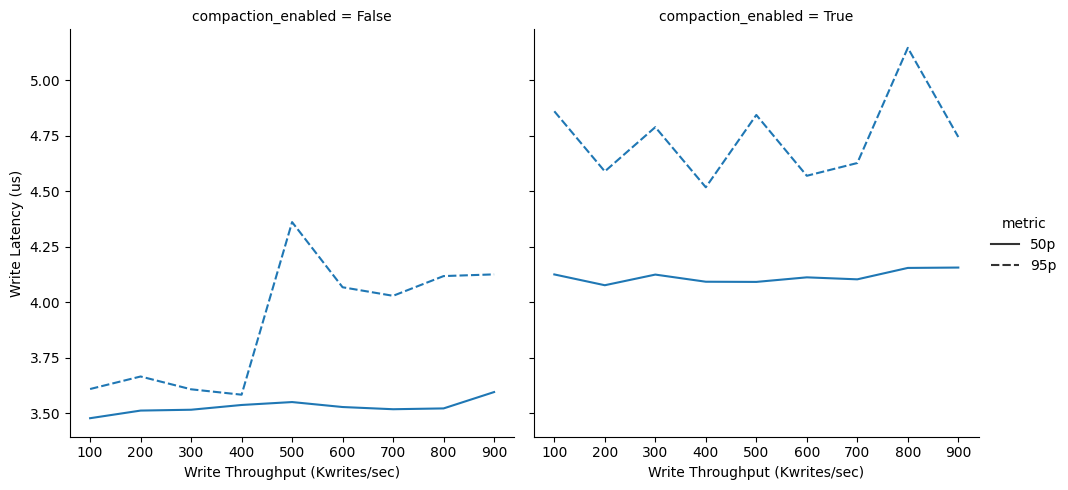
\includegraphics[width=1\textwidth]{compaction_write.png}
    \caption{Write Latency vs Throughput, with Compaction disabled (left) and enabled (right).}
    \label{fig:compaction-write}
\end{figure}

\begin{figure}[h]
    \centering
    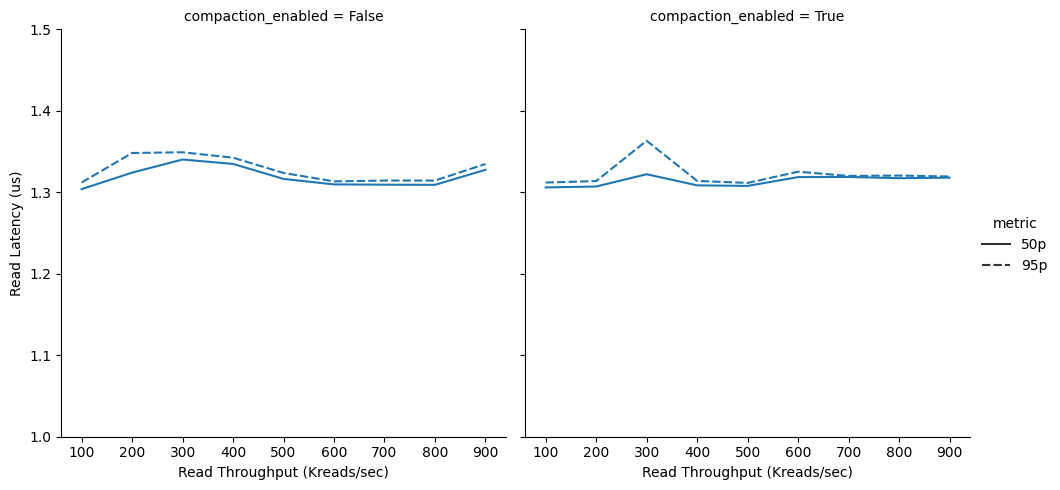
\includegraphics[width=1\textwidth]{compaction_read.png}
    \caption{Read Latency vs Throughput, with Compaction disabled (left) and enabled (right).}
    \label{fig:compaction_read}
\end{figure}

From the experiment results in figures \ref{fig:compaction-write} and \ref{fig:compaction_read} it seems that this is exactly the case. Compaction offers no advantage for reads (which was expected, since file access is still the same), but also neither for writes, which are in fact impaired, as compaction introduces a significant overhead. Therefore, compaction should be avoided in log-structuring.

\subsection{AppendLog}

In AppendLog we only have one tunable parameter, the threshold value, which is the maximum amount of bytes we can write to a runfile before closing it and starting the next one.

This parameter is similar to the \verb"flush_interval" parameter of the HybridLog. When it is too low, frequent merges hinder the write performance, and as it increases, writes on average become faster (because the runfile becomes essentially a large append-only log). However, if the threshold is too high, the files become large and the merges infrequent and cumbersome, which explains the widening of the gap between the 50p and 95p lines in the write latencies in figure \ref{fig:threshold_write_read}. As for the reads, they are not significantly affected, as expected.

\subsubsection{Threshold}

\begin{figure}[h]
    \begin{subfigure}{.5\textwidth}
        \centering
        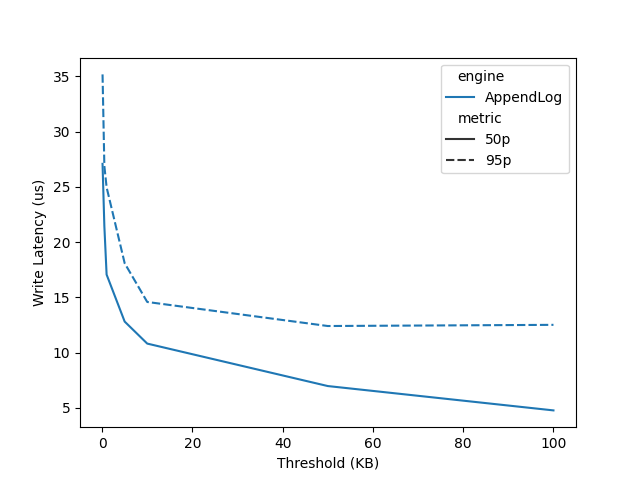
\includegraphics[width=1.1\linewidth]{threshold_write.png}
    \end{subfigure}
    \begin{subfigure}{.5\textwidth}
        \centering
        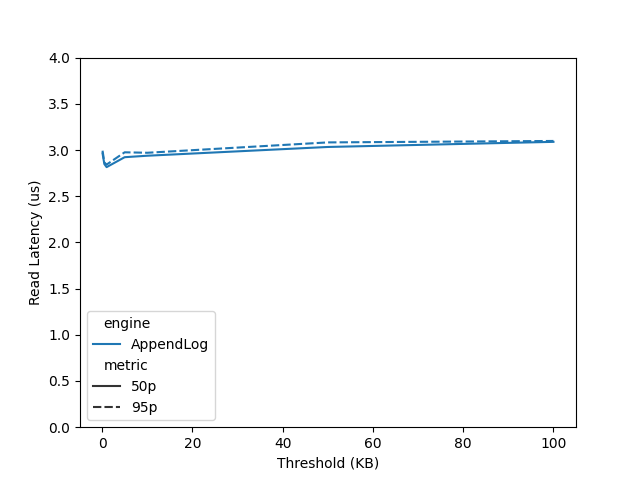
\includegraphics[width=1.1\linewidth]{threshold_read.png}
    \end{subfigure}
    \caption{Latency vs Threshold.}
    \label{fig:threshold_write_read}
\end{figure}

\section{Comparison}

In this section we proceed to compare the engines on their performances when executing the same task with similar parameters. For the following experiments, we use the following parameters: Key and value lengths of 5 bytes each (so 10-byte key-value pairs), $10^5$ unique keys and values, and 10 samples per average latency measurement for the percentiles. Also, for all engines we use \verb"max_runs_per_level="10, for the LSM-Tree \verb"density_factor="10 and \verb"memtable_bytes_limit="100K, for the HybridLog \verb"mem_segment_len="210K, \verb"ro_lag_interval="10K, \verb"flush_interval="10K, and for the AppendLog \verb"threshold="100K.

The above settings lead to almost equally sized files on disk, and use the same configurable memory, so the comparison is fair.

\subsection{Write Latencies}

In figure \ref{fig:comparison-write} we observe the write latencies of each engine as we increase the input throughput. When choosing keys uniformly, HybridLog and AppendLog are significantly faster than the LSM-Tree. This can be attributed to the fast (amortized $O(1)$) hash-based indexing of those engines, versus the LSM-Tree's memtable's data structure, which has an insert complexity of $O(log(n))$. This is also the reason that when we use a state with a size that fits the in-memory structures and therefore does not need to ``spill'' to disk, the HybridLog still performs faster, as can be seen in figure \ref{fig:comparison-write-fit-mem}.

When we choose keys using a Zipfian distribution instead, some keys are accessed compared to the Uniform distribution, the LSM-Tree and the HybridLog become faster than earlier, because the Zipfian distribution allows them to better leverage their in-memory buffering structures before flushing, thus reducing I/O operations, and the AppendLog becomes slower, because it lacks any similar buffering method to take advantage of the Zipfian distribution. Among them, the HybridLog is clearly the fastest, precisely because its memory segment with its fast in-place updates of recently written records exploits the Zipfian distribution best.


\begin{figure}[h]
    \begin{subfigure}{.5\textwidth}
        \centering
        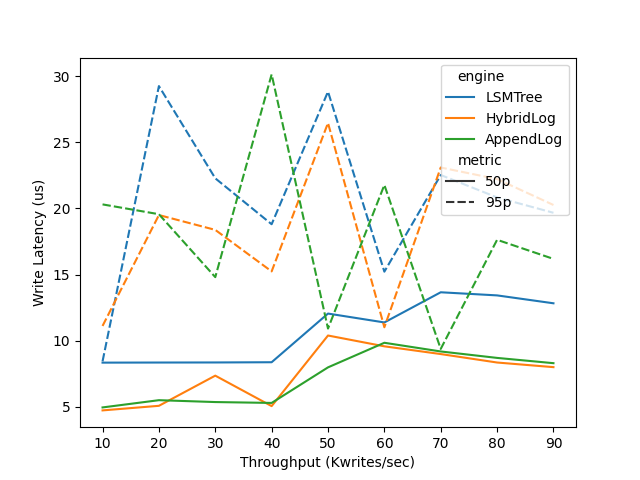
\includegraphics[width=1.1\linewidth]{write-throughput.png}
        \caption{Uniform distribution}
    \end{subfigure}
    \begin{subfigure}{.5\textwidth}
        \centering
        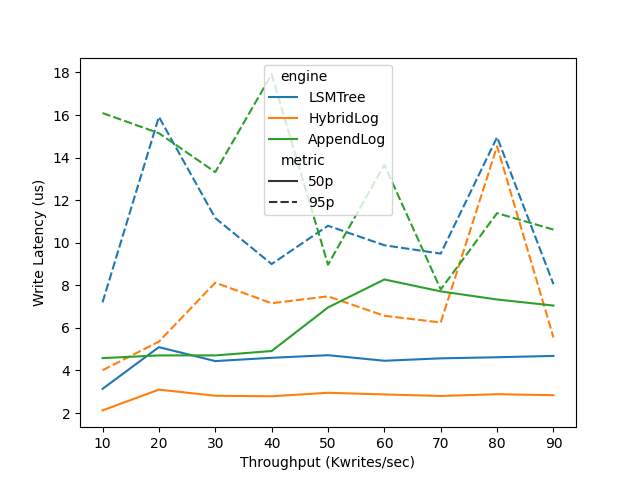
\includegraphics[width=1.1\linewidth]{write-throughput-zipfian.png}
        \caption{Zipfian distribution}
    \end{subfigure}
    \caption{Latency vs Max Runs per Level.}
    \label{fig:comparison-write}
\end{figure}

\begin{figure}[h]
    \centering
    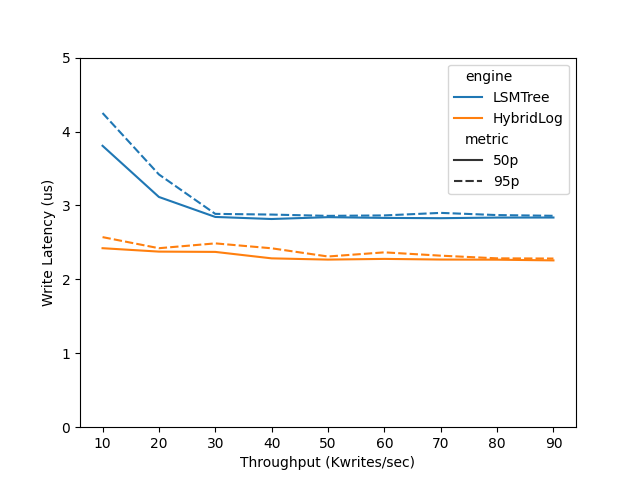
\includegraphics[width=0.6\textwidth]{write-throughput-fit-mem.png}
    \caption{Write Throughtput when data fits the memory}
    \label{fig:comparison-write-fit-mem}
\end{figure}

\subsection{Read Latencies}

Upon examining the latencies for the reads in figure \ref{fig:comparison-read-latencies}, it becomes clear that the HybridLog and AppendLog outperform the LSM-Tree by a large margin. This is because of their fast hash-based in-memory indices and minimal I/O.

\begin{figure}[h]
    \centering
    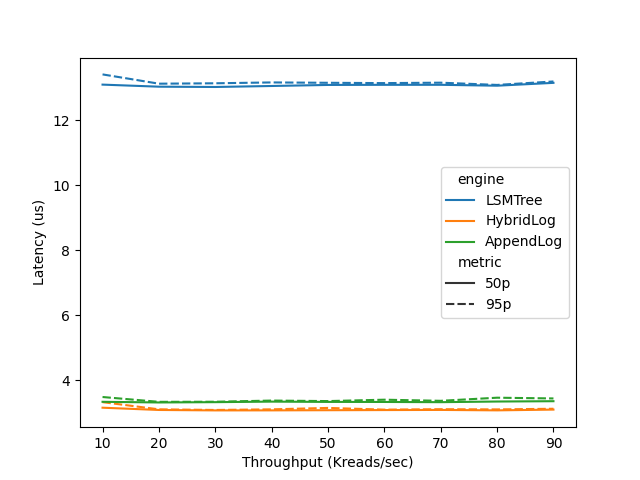
\includegraphics[width=0.6\textwidth]{read-throughput.png}
    \caption{Read Latencies}
    \label{fig:comparison-read-latencies}
\end{figure}

\subsection{Memory}

HybridLog's superiority as the fastest key-value store comes at the cost of high memory usage, as can be seen in figure \ref{fig:comparison-memory}. Indeed, it is the store with the most in-memory structures, including its main index. After that comes the AppendLog, which also keeps its index in memory. Finally, the LSM-Tree uses the least memory of all, making it ideal for low-memory environments (and also the cheaper option). The components requiring memory in the LSM-Tree are the Bloom filters and the fence pointers, which we keep in memory for fast access.

\begin{figure}[h]
    \centering
    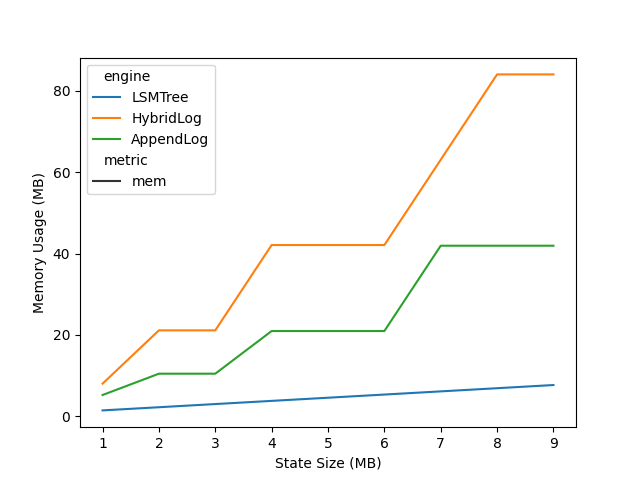
\includegraphics[width=0.6\textwidth]{mem.png}
    \caption{Memory Usage}
    \label{fig:comparison-memory}
\end{figure}

\section{Incremental Snapshotting}

This section focuses on evaluating the incremental snapshotting capabilities of the three log-structured engines. Towards this goal, to demonstrate the advantage of having incremental snapshots, we compare the LSM-Tree, HybridLog and AppendLog to ``MemOnly'', which is a naive implementation of a key-value store based on an entirely in-memory hosted HashMap that dumps its whole state to disk every time we want to take a snapshot of it.

We do two experiments. In the first, we iterate and write new key-value pairs, taking also a snapshot at the end of each iteration. In the second experiment, we first perform a large write-volume of 1GB, and then we write data in small increments on 1KB, taking a snapshot after each increment.

For both experiments, we use keys and values of 2 and 8 bytes respectively so that the available keys are no more than $2^{16}$ and therefore we will not need too much memory for the indices of HybridLog, AppendLog and MemOnly. Also, to simulate a snapshot over the network, we add an overhead of 1$\mu$s per byte (as if we had a network channel of 1MB/s). The settings for all engines are similar so that the comparison is as fair as possible.

The results of the first experiment are shown in figure \ref{fig:snapshot}. As expected, the naive MemOnly database dumps the whole state at every step, leading to a quadratic increase of the total time taken to take $n$ snapshots, while the other log-structured stores increase linearly. During each snapshotting step, they only dump the new inserts, except from a few cases when some merging takes place and have to push some larger files as well, but still, they perform better than MemOnly.

For the second experiment, where only updates take place, the results can be seen in figure \ref{fig:snapshot-static-state}. Again, as expected, the LSM-Tree, HybridLog and AppendLog only push the updates, while the MemOnly store pushes the whole state every time. By observing the cumulative graph, it is evident that the log-structured stores take snapshots more efficiently than the naive method.

\begin{figure}[h]
    \begin{subfigure}{.5\textwidth}
        \centering
        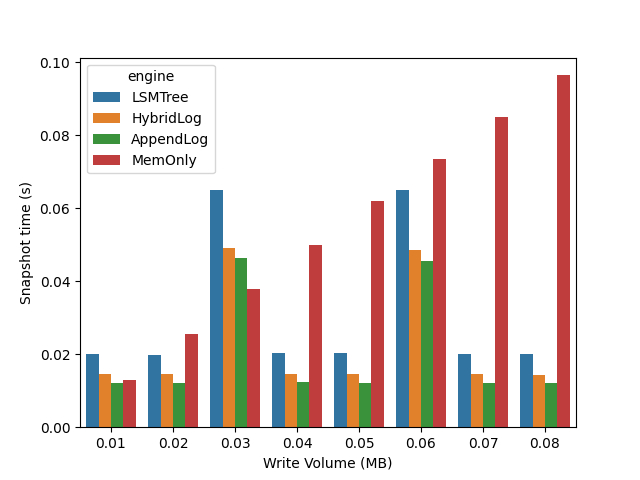
\includegraphics[width=1.1\linewidth]{snapshot.png}
        \caption{Discrete}
    \end{subfigure}
    \begin{subfigure}{.5\textwidth}
        \centering
        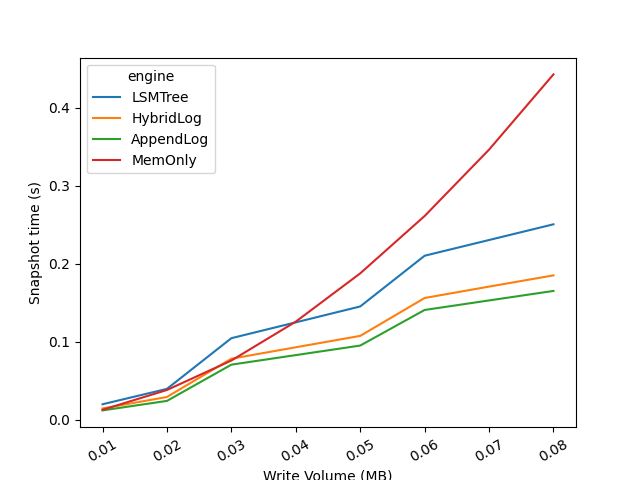
\includegraphics[width=1.1\linewidth]{snapshot-aggr.png}
        \caption{Cumulative}
    \end{subfigure}
    \caption{Snapshotting Time vs Write Volume, when we increase the state by inserting new records.}
    \label{fig:snapshot}
\end{figure}

\begin{figure}[h]
    \begin{subfigure}{.5\textwidth}
        \centering
        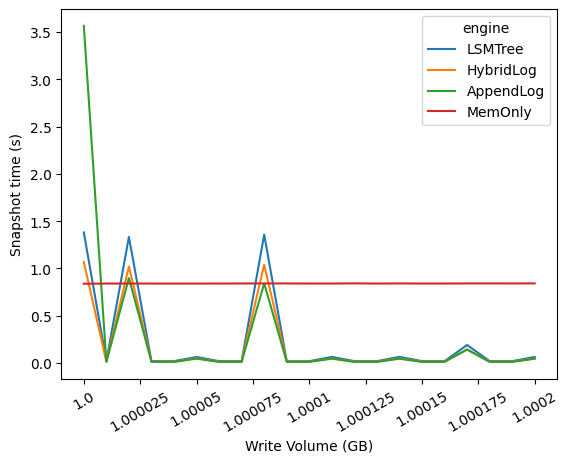
\includegraphics[width=1.1\linewidth]{snapshot-static-state.png}
        \caption{Discrete}
    \end{subfigure}
    \begin{subfigure}{.5\textwidth}
        \centering
        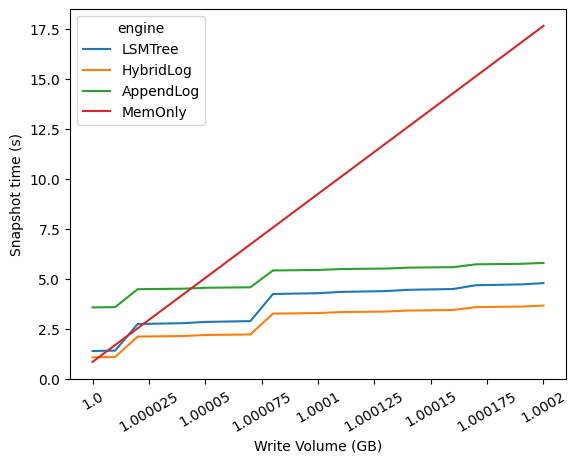
\includegraphics[width=1.1\linewidth]{snapshot-static-state-aggr.png}
        \caption{Cumulative}
    \end{subfigure}
    \caption{Snapshotting Time vs Write Volume, when state stays the same and we only update it.}
    \label{fig:snapshot-static-state}
\end{figure}

The important takeaway from these two experiments is that while the cumulative time of the naive snapshotting method increases quadratically at the worst case, the log-structured incremental methods increase linearly. This distinction can have significant ramifications in the performance of systems that keep large states.

% \section{Discussion}

% TODO table with advantages and disadvantages of each kvstore. 
%!TEX root = ../main.tex

\chapter{Conclusion}

\label{Chapter5-conclusion}

\section{Summary}

In this work, we have implemented three different key-value stores, as state backends that support incremental snapshotting in transactional dataflow SFaaS systems.
We analyzed their behavior and the trade-offs governing their operation under different settings of their parameters, gaining insight on how they should be tweaked to deliver the best performance according to the use case.
Then, we performed fair comparisons between them, indicating the strengths and weaknesses of each and the domains on which each of them excels.
Finally, we implemented logic to support incremental snapshotting capabilities and rollback to previous versions, and evaluated this as well.

% TODO answer research questions

\section{Future Work}

TODO
% let the programmer choose, check to paper "in support of workload-aware..."

% all works tweak log-structuring for either reads or writes. proposal: optimize for snapshot and state recovery
 

%----------------------------------------------------------------------------------------
%	THESIS CONTENT - APPENDICES
%----------------------------------------------------------------------------------------

\appendix % Cue to tell LaTeX that the following "chapters" are Appendices

% Include the appendices of the thesis as separate files from the Appendices folder
% Uncomment the lines as you write the Appendices

%!TEX root = ../main.tex

% Appendix Template

\chapter{Code} % Main appendix title

\label{Appendix-A-code} % Change X to a consecutive letter; for referencing this appendix elsewhere, use \ref{AppendixX}

\section{Key-value store API}

\begin{lstlisting}[language=Python, caption=Key-value store API - method signatures.]
class KVStore:
    def __getitem__(self, key: bytes) -> bytes:
        pass

    def __setitem__(self, key: bytes, value: bytes) -> None:
        pass

    def get(self, key: bytes) -> bytes:
        pass

    def set(self, key: bytes, value: bytes) -> None:
        pass

    def __sizeof__(self) -> int:
        pass

    def close(self) -> None:
        pass

    def snapshot(self) -> None:
        pass

    def restore(self, version: Optional[int] = None) -> None:
        pass
\end{lstlisting}

\section{Replica API}

\begin{lstlisting}[language=Python, caption=Replica API - method signatures.]
class Replica:
    def put(self, filename: str) -> None:
        pass

    def get(self, filename: str, version: int = None):
        pass

    def gc(self):
        pass

    def restore(self, max_per_level: int, version: int = None):
        pass

    def destroy(self):
        pass
\end{lstlisting}

\begin{lstlisting}[language=Python, caption=Algorithm used in snapshot rollback.]
def expand_version(version: int, max_per_level: int) -> list[tuple[int, int]]:
    acc = []
    while version != 0:
        acc.append(version % max_per_level)
        version //= max_per_level

    levels_runs = []
    for i, e in enumerate(acc):
        j = e - 1
        while j >= 0:
            levels_runs.append((i, j))
            j -= 1

    return levels_runs
\end{lstlisting}

%%!TEX root = ../main.tex

% Appendix Template

\chapter{Experiments on HDD drives} % Main appendix title
\label{Appendix-B} % Change X to a consecutive letter; for referencing this appendix elsewhere, use \ref{AppendixX}

The following experiments were conducted in an HDD drive which was benchmarked to have a random-write bandwidth of 1.2 MB/s and a sequential-write bandwidth of 2.7 MB/s with the \verb|fio| tool.

The intention behind conducting this experiment was to evaluate whether slower rotational magnetic hard drives can influence the results in Chapter \ref{Chapter4-evaluation}. The experiments in Chapter \ref{Chapter4-evaluation} were conducted in an NVMe SSD drive which is faster and non-rotational.

It seems that these characteristics do not have an impact on the outcome. The diagrams are visually similar (because the random seeds are the same), they are just ``shifted slightly upwards'' because the drive is slower.

The absence of any significant difference in the results can be justified by the fact that all stores write data sequentially, not randomly, and sequential writes are similar to both types of drives in the sense that they are both fast. It's random writes that degrade the performance of rotational HDDs because the disk head must move and wait for the disk to rotate, and this type of writes is not common in our implementations.

\section{Compaction in AppendLog}

\begin{figure}[h]
    \centering
    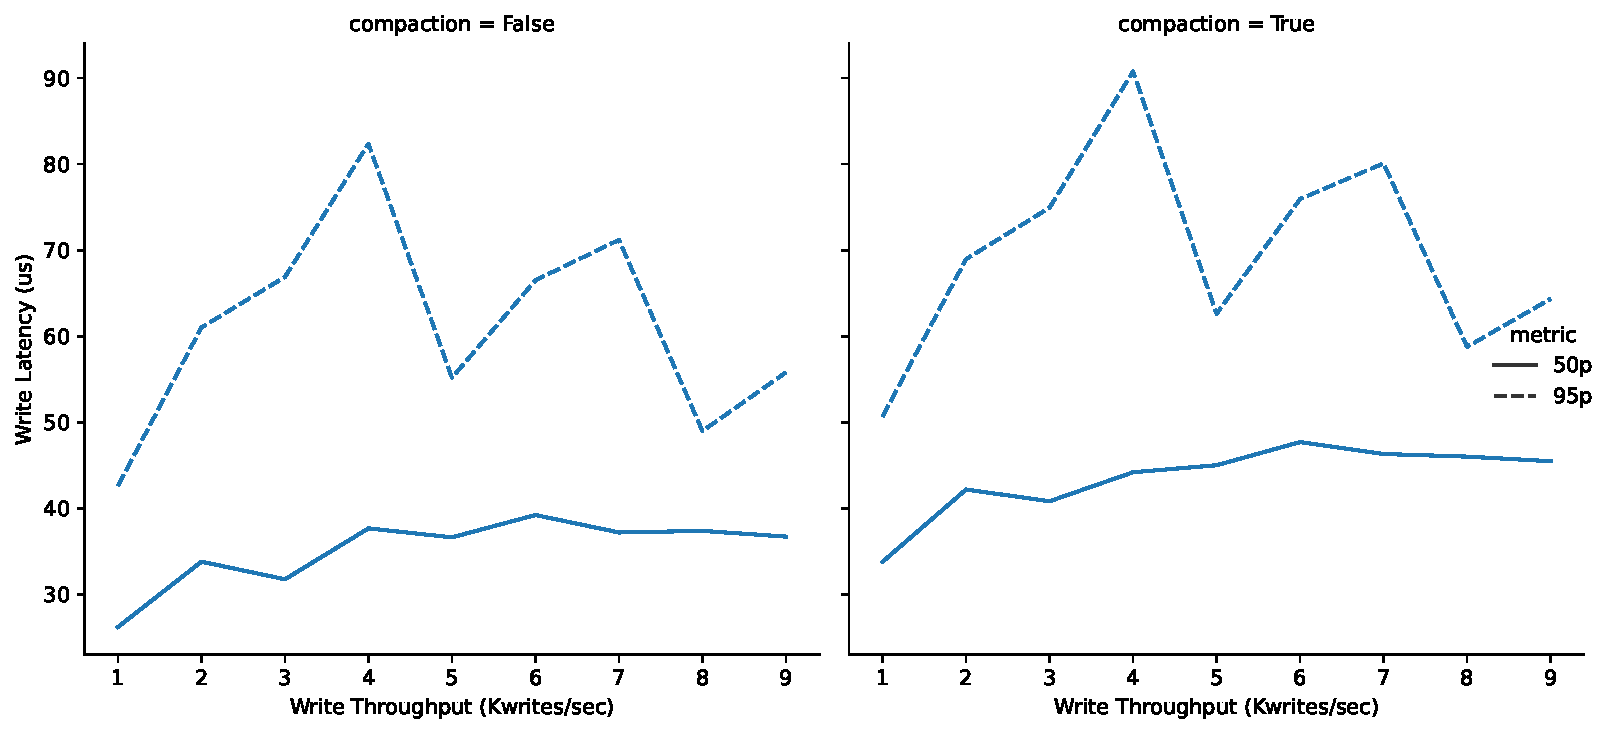
\includegraphics[width=1\textwidth]{compaction_write-hdd.pdf}
    \caption{Writes in AppendLog with compaction disabled (left) and enabled (right) in an HDD.}
    \label{fig:compaction-write-hdd}
\end{figure}

\begin{figure}[h]
    \centering
    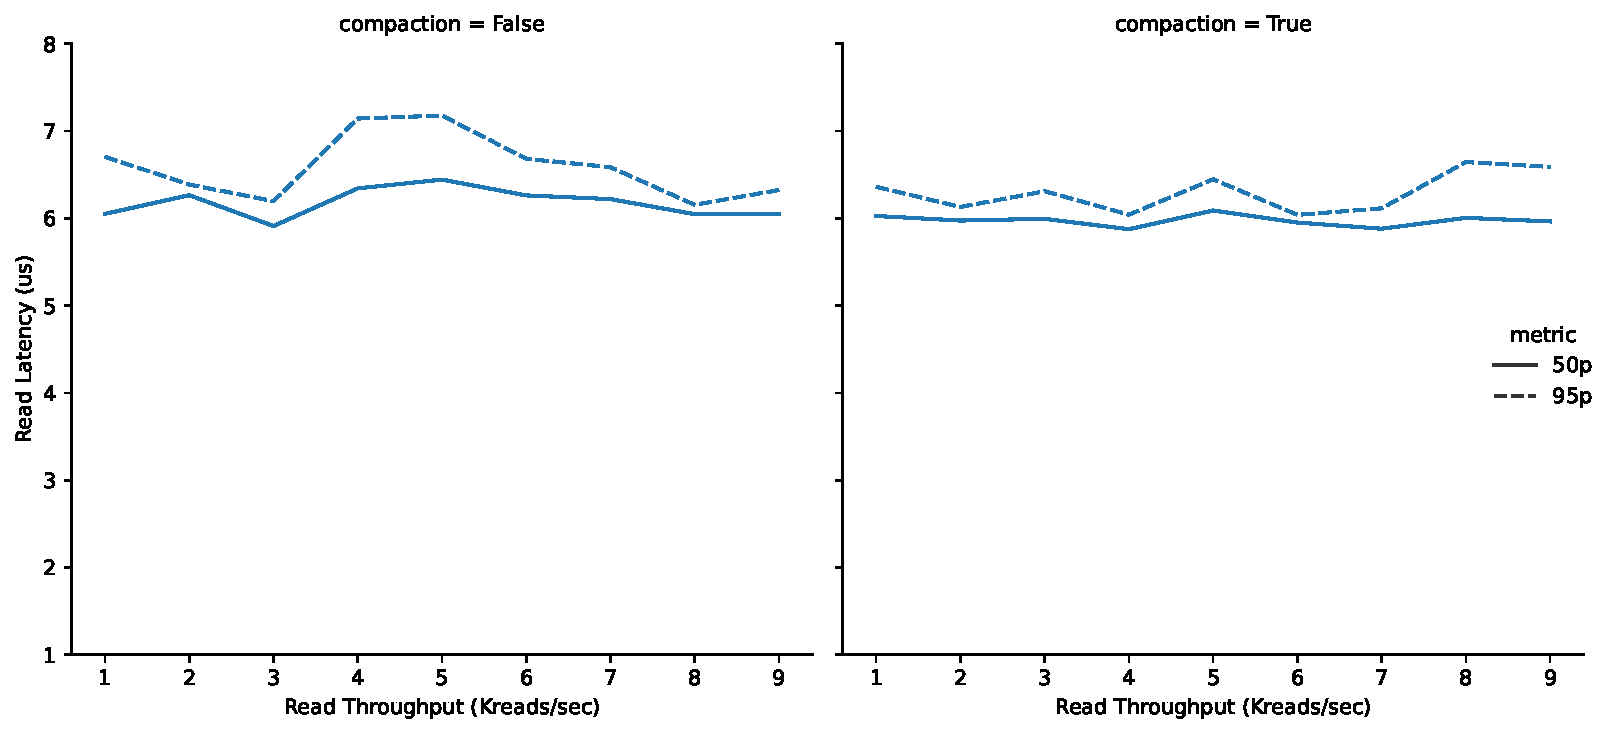
\includegraphics[width=1\textwidth]{compaction_read-hdd.pdf}
    \caption{Reads in AppendLog with compaction disabled (left) and enabled (right) in an HDD.}
    \label{fig:compaction-read-hdd}
\end{figure}

\section{Latencies}

\begin{figure}[h]
    \centering
    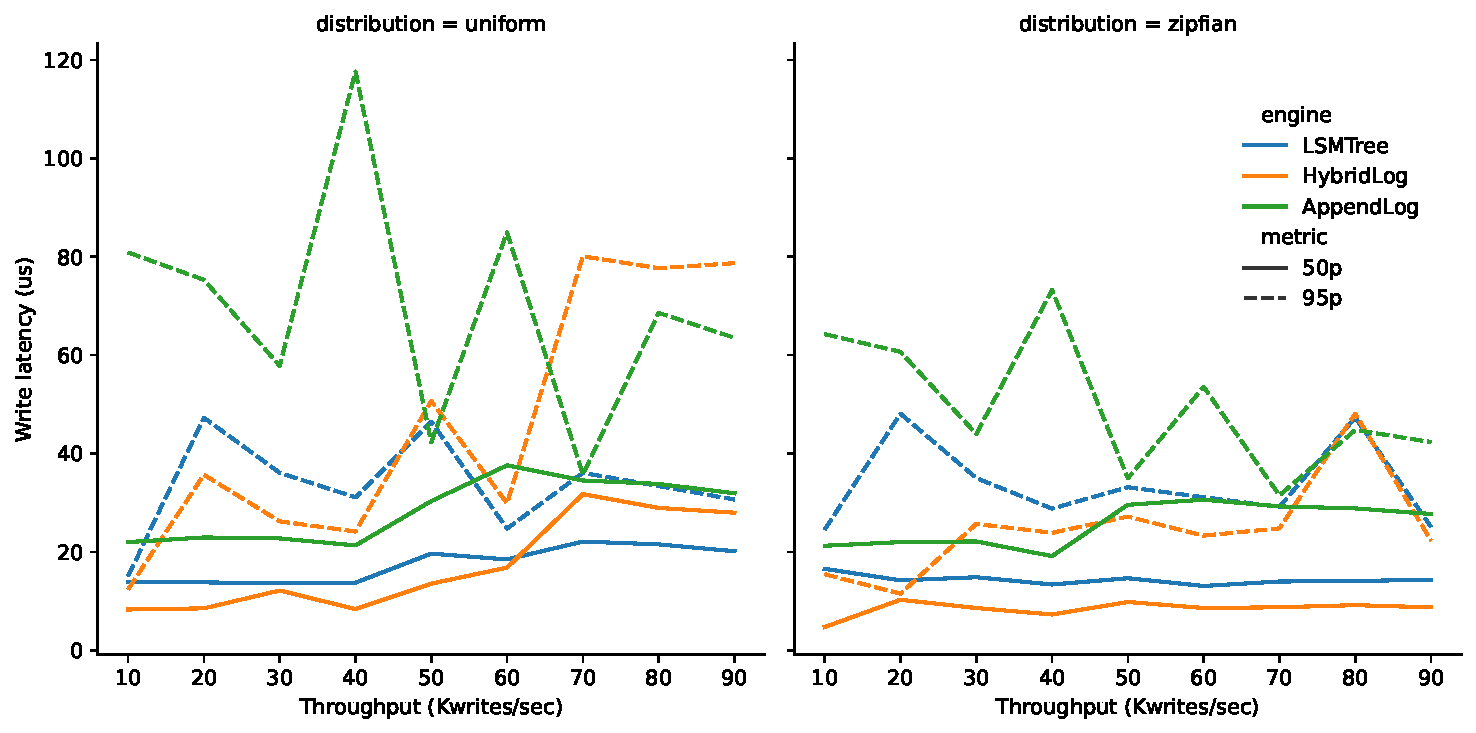
\includegraphics[width=1\textwidth]{write-throughput-hdd.pdf}
    \caption{Write latency for every store in an HDD.}
    \label{fig:write-throughput-hdd}
\end{figure}

\begin{figure}[h]
    \centering
    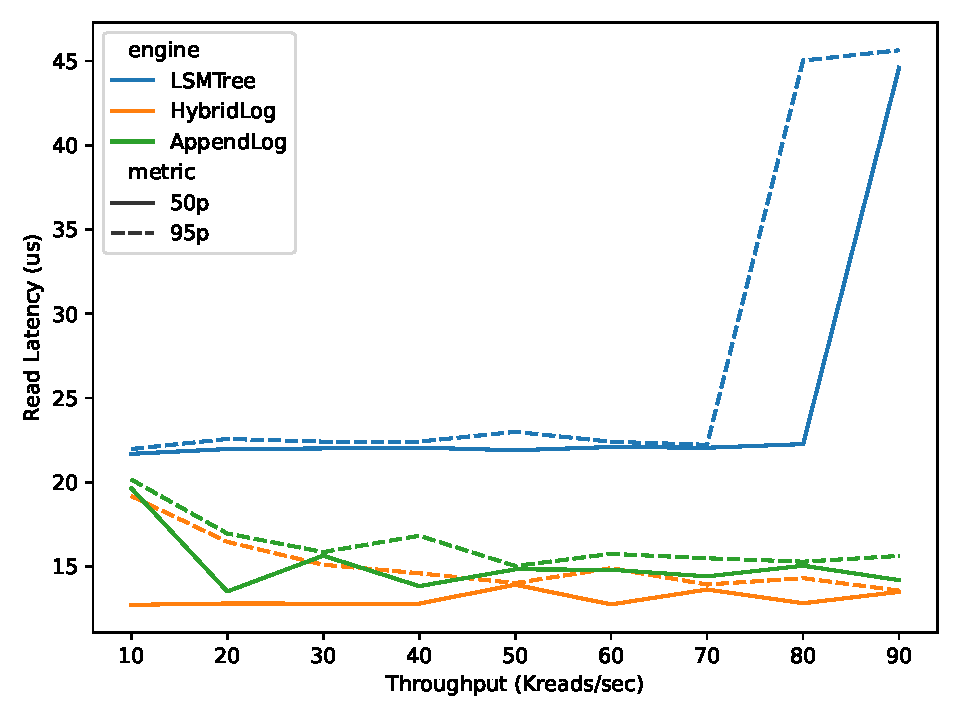
\includegraphics[width=0.6\textwidth]{read-throughput-hdd.pdf}
    \caption{Read latency for every store in an HDD.}
    \label{fig:}
\end{figure}

%\include{Appendices/AppendixC}

%----------------------------------------------------------------------------------------
%	BIBLIOGRAPHY
%----------------------------------------------------------------------------------------

\printbibliography[heading=bibintoc]

%----------------------------------------------------------------------------------------

\end{document}  
